\subsubsection*{Elektrische Spannung}
        Inhomogen:
        \mathbox{U = \Phi(P) - \Phi(P_0) = -\int\limits_{P_0}^{P} \overrightarrow{E}\overrightarrow{ds}} 
        Beispiel Punktladung:

        %\vspace{-1mm}
        %\begin{minipage}{0.53\linewidth}
        %    \begin{footnotesize}
        %        \begin{center}
        %            \mathbox{
        %                U = \int_{1}^{2}\overrightarrow{E}(r)\:\overrightarrow{dr}            }
        %        \end{center}
        %    \end{footnotesize}
        %\end{minipage}
        %\vspace{1mm}
        %\begin{minipage}{0.46\linewidth}
        %    \begin{scriptsize}
        %        \begin{center}
        %            \begin{align*}
        %                \overrightarrow{E}\text{(r), } &\text{E-Feld wird gegen aussen}
        %                \\ &\text{schwächer}
        %            \end{align*}
        %            \begin{align*}
        %                \Phi &= \text{Potential} [V]
        %            \end{align*}
        %        \end{center}
        %    \end{scriptsize}
        %\end{minipage}

        \vspace{-1mm}
            \begin{minipage}{0.41\linewidth}
                \begin{footnotesize}
                    \begin{center}
                        \vspace{2mm}
                        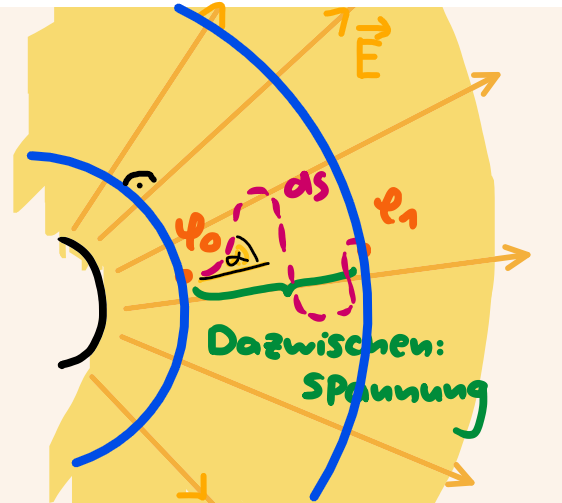
\includegraphics[width = 27mm]{src/images/inhom_potentialfeld.png}
                    \end{center}
                \end{footnotesize}
            \end{minipage}
            \begin{minipage}{0.58\linewidth}
                \begin{scriptsize}
                    \begin{center}
                        \begin{empheq}[box = \fbox]{align*}
                        %\mathbox{
                            U &= \int_{1}^{2}E\cdot\cos (\alpha) ds\\
                            &= \int_{1}^{2}\overrightarrow{E}(r)\:\overrightarrow{dr}
                        \end{empheq}
                        Auf \colorbox{Cyan}{Kreis $\Phi_{0/1}$} stets selbes Potential/Spannung
                    \end{center}
                \end{scriptsize}
            \end{minipage}
            \vspace{2mm}
            
        Homogen:

        \vspace{-1mm}
            \begin{minipage}{0.41\linewidth}
                \begin{footnotesize}
                    \begin{center}
                        \vspace{2mm}
                        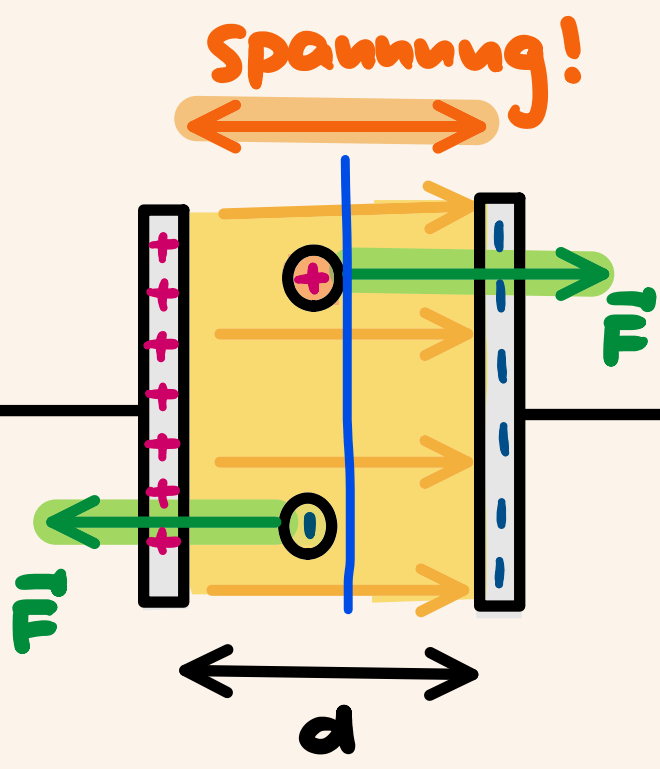
\includegraphics[width = 27mm]{src/images/hom_potentialfeld.png}
                    \end{center}
                \end{footnotesize}
            \end{minipage}
            \begin{minipage}{0.58\linewidth}
                \begin{scriptsize}
                    \begin{center}
                        \mathbox{
                            U = E\cdot d
                        }
                        Auf \colorbox{Cyan}{Linie} stets selbes Potential/Spannung
                    \end{center}
                \end{scriptsize}
            \end{minipage}
            \vspace{1mm}